\chapter{Compacidad}%
\label{cha:compacidad}
\section{Concepto y mantras}%
\label{sec:concepto_y_mantras_comp}
\begin{defi}
$X$ es \textbf{compacto} si todo recubrimiento abierto tiene un subrecubrimiento finito:
\[
X = \bigcup_{i \in  I} U_i \Rightarrow \exists U_{i_1} \cup \ldots \cup U_{i_r} = X
\]
\end{defi}

\begin{obs}[Propiedad de la intersección finita]
Complementando lo anterior tenemos:
\begin{gather*}
    \emptyset = \bigcap_{i \in I} F_i \Rightarrow \exists F_{i_1} \cap \ldots \cap F_{i_r} = \emptyset \Rightarrow\\
    \boxed{    \forall F_{i_1} \cap \ldots \cap F_{i_r} \neq \emptyset \Rightarrow \bigcap_{i \in  I} F_i \neq \emptyset}
.\end{gather*}
\end{obs}

\begin{prop}[Subespacios]
Sea $K \subset X$ (compacto) $\Rightarrow K \subset \bigcup_{i \in  I} U_i$ con $U_i \ab X \Rightarrow \exists U_{i_1} \cup \ldots \cup U_{i_r} \supset K$
\end{prop}

\begin{ej}
\begin{enumerate}
    \item $K \subset \mathbb{R}_u^n$ es compacto $\Leftrightarrow K$ es cerrado y acotado (Heine-Borel). 
    \item $\left[ a, b \right] \subset \mathbb{R}_u$ compacto. ($\Rightarrow$ Heine-Borel por resultados generales).
    \item Si $X$ es compacto con $\mathcal{T}_{\text{discr.}} \Rightarrow$ es finito 
    \begin{demo}
        $X = \bigcup_{x \in X} \{x\}$ es recubrimiento abierto en $\mathcal{T}_{\text{discreta}}$ y como es compacto $\exists \bigcup_{i=1}^n \left\{ x_i \right\} = X$.
    \end{demo}
    \item $x_k \rightarrow x \Rightarrow K = \{x, x_k: k \ge 1\}$ es compacto.
    \begin{demo}
        \[
            \exists U_{i_0}^x \ni x \xRightarrow{\lim} \begin{rcases}
                x_k \in U_{i_0},\ \forall k > k_0\\
                x_k \in U_{i_k},\ \forall k \le k_0
            \end{rcases} \Rightarrow K \subset U_{i_0} \cup U_{i_1} \cup \ldots \cup U_{i_{k_0}} 
        \]
    \end{demo}

    \item $K \subset \mathbb{R}_u^n$ compacto $\Leftrightarrow \forall A^{\infty} \subset K, A' \cap K \neq \emptyset$ (Bolzano-Weierstrass)
\end{enumerate}
\end{ej}

\begin{prop}[Mantra 1]
Cerrado en compacto es compacto. 
\end{prop}
\begin{demo}
Sea $K \cerr X = \bigcup U_i$,
\begin{align*}
    K \subset \bigcup U_i &\Rightarrow X = \left( X \setminus K \right) \cup \bigcup U_i\\
    X \text{ compacto} &\Rightarrow \exists \left( X \setminus K \right) \cup U_{i_1} \cup \ldots \cup U_{i_r} = X \supset K\\
    &\Rightarrow U_{i_1} \cup \ldots \cup U_{i_r} \supset K
.\end{align*}

(Alternativa: Usar la propiedad de las intersecciones finitas)
\end{demo}

\begin{prop}[Mantra 2]
Infinito en compacto tiene puntos de acumulación.
\end{prop}
\begin{demo}
Sea $A \subset X$ (compacto) con $A' = \emptyset$ veamos que es finito:
\begin{align*}
    \overline{A} &= \overbrace{\{\text{puntos aislados}\}}^{\subset A} \cup \cancelto{\emptyset}{A'} = \{\text{puntos aislados}\} = A\\
     &\Rightarrow A \cerr X \text{ comp.} \Rightarrow A \text{ es compacto y discreto} \Rightarrow \#A < +\infty   
.\end{align*}
El resultado del enunciado lo podemos sacar por el contrarrecíproco.
\end{demo}

\begin{obs}
Este mantra es como ``la mitad'' del teorema de Bolzano-Weierstrass.
\end{obs}

\begin{prop}[Mantra 3]
La imagen continua de un compacto es compacta. 
\end{prop}
\begin{demo}
Sea $f: X \rightarrow Y$ con $f$ continua y $X$ compacto $\Rightarrow$
\begin{align*}
    f\left( X \right) \subset \bigcup_{i} V_i &\Rightarrow X = \bigcup_{i} f^{-1} V_i \Rightarrow \exists f^{-1}V_{i_1} \cup \ldots \cup f^{-1}V_{i_r} = X\\
     &\Rightarrow V_{i_1} \cup \ldots \cup V_{i_r} \supset f\left( X \right) 
.\end{align*}
\end{demo}

\begin{ej}[¡Muy importante!]
$\mathbb{R} \mathrm{P}^n$ es compacto al ser la imagen continua de $\mathbb{S}^n$ por la \underline{proyección antipodal}. 
\end{ej}

\begin{prop}[Mantra 4]
Un compacto en $T_2$ es cerrado. 
\end{prop}
%TODO: No estoy seguro que es cada cosa.
\begin{demo}
Vamos a ver que $X \setminus K$ es abierto al ser entorno de todos sus puntos.

Sea $K \subset X$ con $K$ compacto y $X$ Hausdorff $\Rightarrow$
\begin{equation} \label{eq:mantra_4_1}
    \forall x \in X \setminus K,\ \exists U^x \cap U^K = \emptyset
\end{equation}

Porque $\forall y \in K,\ \exists U_y^x \cap U^y = \emptyset$ por $T_2 \Rightarrow$
\begin{align*}
    %TODO: Fix flecha
    K \subset \bigcup_{y} U^y &\xRightarrow{\text{comp.}} K \subset U^{y_1} \cup \ldots \cup U^{y_r} = U^K\\
    &\xRightarrow{\text{comp.}} x \in U_{y_1}^x \cap \ldots \cap U_{y_r}^x = U^x
.\end{align*}
Finalmente, utilizando \ref{eq:mantra_4_1} $\Rightarrow$
\[
    U^x \subset X \setminus K\; \land \;X\setminus K \text{ es entorno de } x \Rightarrow X \setminus K \text{ abierto.} 
\]
%TODO: Imagen
\begin{center}
    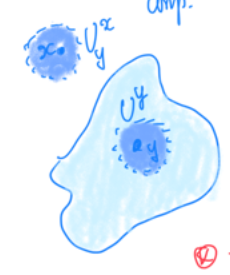
\includegraphics[scale=0.3]{images/mantra_4} 
\end{center}
\end{demo}
\begin{coro}
Dos compactos disjuntos en un $T_2$ se separan como puntos.
\end{coro}
\begin{demo}
    Ejercicio usando \ref{eq:mantra_4_1}.
\end{demo}

\begin{prop}
Si $f : X \rightarrow Y$ es continua, $X$ compacto e $Y$ Hausdorff $\Rightarrow f$ es cerrada.
\end{prop}
\begin{demo}
Sea $F \cerr X \xRightarrow{\text{M1}}$
\[
    F \text{ comp.} \xRightarrow{\mathrm{M}3} f\left( F \right) \text{ comp.} \xRightarrow{\mathrm{M}4} f\left( F \right) \text{ cerr.} 
\]
\end{demo}
\begin{coro}
Sea la $f$ de la anterior proposición entonces si además es:
\[
\begin{cases}
    \text{inyectiva}\\
    \text{sobreyectiva}\\
    \text{biyectiva}
\end{cases} \Rightarrow
\begin{cases}
    \text{inmersión cerrada}\\
    \text{identificación cerrada}\\
    \text{homeomorfismo}
\end{cases} 
\]
\end{coro}

\section{Tabla de comportamiento}%
\label{sec:tabla_de_comportamiento_comp}
%TODO: Fix tabla
\begin{table}[H]
\centering
\begin{tabular}{| c | c | c | c | c |}
\hline
& Subespacios & Cocientes & Productos & Sumas\\
\hline
    Compacidad & \begin{tabular}{@{}c@{}}$\times$\\ cerrados \checkmark \end{tabular} & \checkmark & \checkmark & \checkmark\\
\hline
    & Mantra $1$ & Mantra $3$ & Tychonoff & Unión finita\\
\hline
\end{tabular}
\caption{\textit{La tabla nos indica como se mantiene (o no) la compacidad con las distintas construcciones que hemos visto. La última fila nos indica la demostración, o contraejemplo, de cada una.}}
\end{table}

\begin{theo}[de Tychonoff]
Si $X$ e $Y$ son dos compactos $\Rightarrow X \times Y$ es compacto.
\end{theo}
\begin{demo}
Sea $X \times Y = \bigcup_{i \in  I} W_i,\ W_i \in \mathcal{T}_X \times \mathcal{T}_Y$.
\begin{enumerate}
    \item $\forall x\ \forall y,\ \exists U_y^x \times V_x^y \subset W_i$, $i$ depende de $\left( x, y \right)$.
    \item $\forall x\ Y = \bigcup_{y} V_x^y \xRightarrow{Y \text{comp.}} Y = V_x^{y_1} \cup \ldots \cup V_x^{y_r}$, los $y_k$ y su nº dependen de $x$.
    \item $U^x = U_{y_1}^x \cap \ldots \cap U_{y_r}^x,\ U^x \times V_x^{y_k} \subset W_{i_k}$, $i_k$ depende de $x$.
    \item $X = \bigcup_{x} U^x \xRightarrow{X \text{comp.}} X = U^{x_1} \cup \ldots \cup U^{x_s}$.
    \item 
    \[
        X \times Y = \bigcup_{\substack{l, k\\ \text{fin.}}} U^{x_l} \times V_{x_l}^{y_k} \subset \bigcup_{\substack{l, k\\ \text{fin.}}} W_{i_k} \text{, los } i_k \text{ dependen de los } x_l. 
    \]
\end{enumerate}
\end{demo}

\begin{obs}
\begin{enumerate}
    \item $X \times Y$ compacto $\Rightarrow X$ e $Y$ compactos.\begin{demo}
        Aplicamos el Mantra $3$ para las proyecciones.
    \end{demo} 
    \item Heine-Borel: $K \subset \mathbb{R}_u^n$ cerrado y acotado $\Rightarrow$ compacto.
    \begin{demo}
    Ya que sabemos que $\left[ a, b \right]$ es compacto en $\mathbb{R}_u$, sabemos que:
    \[
        \exists a_i, b_i: K \cerr \underbrace{\left[ a_1, b_1 \right] \times \ldots \times \left[ a_n, b_n \right]}_{\text{Compacto por Tych.}}  
    \]
    y aplicamos el Mantra $1$.
    \end{demo}
\end{enumerate}
\end{obs}


\chapter{Compacidad local}%
\label{cha:compacidad_local}
\begin{defi}
Sea $Y \subset X$, es \underline{localmente cerrado} si cumple las condiciones equivalentes siguientes:
\begin{enumerate}
    \item $\forall y \in Y,\ \exists U^y \subset X: Y \cap U^y \cerr U^y$. ($\Rightarrow$ lo mismo $\forall V^y \subset U^y$)
    \item $Y$ es abierto en su adherencia.
    \item $Y = F \cap U,\ F \cerr X,\ U \ab X$. ($\Rightarrow$ vale $F = \overline{Y}$)
\end{enumerate}
\end{defi}
\begin{demo}
\begin{enumerate}
    \item[1. $\Rightarrow$ 2.)] $Y = \overline{Y} \cap \left( \bigcup_{y \in Y} U^y \right)$:
    \begin{align*}
        x \in \overline{Y} \cap U^y &\Rightarrow x \in \adh_{U^y} \left( Y \cap U^y \right) = Y \cap U^y \subset Y\\
        U^x \subset U^y &\Rightarrow \emptyset \neq Y \cap U^x = \left( Y \cap U^y \right) \cap U^x
    .\end{align*}
    \item[2. $\Rightarrow$ 3.)] Abierto en $\overline{Y} = \underbrace{\overline{Y}}_{= F} \cap U$.
    \[
    F \cap U = Y \Rightarrow F \supset \overline{Y} \Rightarrow F \cap U = \overline{Y} \cap U.
    \]
    \item[3. $\Rightarrow$ 1.)] $Y = F \cap U \cerr U \left( = U^y,\ \forall y \right)$.
\end{enumerate}
\end{demo}

Esto es un ejemplo de \underline{localización} de una propiedad topológica $\mathcal{P}$ (aquí es ser cerrado). Se puede entender como:
\begin{align*}
    &\forall x,\ \exists V^x \text{ que cumple } \mathcal{P} \text{ o } \\
    &\forall x,\ \exists \mathcal{V}^x \text{ base de entornos que cumplen } \mathcal{P} 
.\end{align*}
A veces son equivalentes (como en este caso), a veces no. El concepto adecuado de localización es mediante \underline{bases de entornos}.

\section{Compacidad local y mantras}%
\label{sec:compacidad_local_y_mantras}
\begin{defi}
$X$ es \underline{localmente compacto} si $\forall x \in X,\ \exists \mathcal{V}^x$ base de entornos compactos.
\end{defi}

\begin{ej}
\begin{enumerate}
    \item $\mathbb{R}_u^n$ es localmente compactos: $\mathcal{V}^x = \{B\left[ x, \varepsilon \right] : \varepsilon > 0\}$

    \item $T = B\left( 0, 1 \right) \cup \{p\},\ T_u$ no es compacto:
    \begin{align*}
        \exists V^p \stackrel{\text{comp.}}{\subset} T &\Rightarrow \exists B\left( 0, \varepsilon \right) \cap T \subset V^p \Rightarrow \exists \overbrace{x_k}^{\in V^p} \rightarrow x_0 \in S\left( 0, 1 \right) \setminus T\\
       &\Rightarrow \{x_k : k \ge 1\} \subset V^p \subset T 
    .\end{align*}
    que es un conjunto infinito sin acumulación en $T$.
    %TODO: Imagen
    \begin{center}
        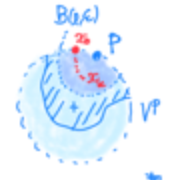
\includegraphics[scale=0.3]{images/loc_comp_ej_2} 
    \end{center}

    \item En general \underline{no} basta que exista un entorno compacto.

    %TODO: no sé que pone
    En $S = T \cup \{q\}?$ tomamos como entornos del punto añadido $q$ los $W \subset S$ que tienen complementario finito (y $q \in W$).

    Pero este caso es un ejemplo con un espacio \underline{no separado}.
\end{enumerate}
\end{ej}

\begin{prop}
Si $X$ es $T_2$ y $x \in X$ tiene un entorno compacto, entonces tiene una base de entornos compactos.
\end{prop}
\begin{demo}
    $\exists \underbrace{V^x}_{\supset W^x \text{ab.}}$ compacto $\Rightarrow \mathcal{V}^x =$ { entornos compactos $K^x$} \underline{base de entornos}: $\forall U^x,\ \exists?K^x \subset U^x$.

    $\exists_{\text{ab.}} U_1^x \subset \overline{U_1^x} \subset U^x$:
    \begin{gather*}
        V^x\setminus U^x \cerr V_{\text{comp.}}^x \Rightarrow \overbrace{V \setminus U}^{\not\ni x} \text{comp. en } T_2 \Rightarrow \exists \overbrace{U_1^x\ \&\ A}^{\text{ab. disjuntos}} \supset V^x \setminus U^x\\
        K^x = \overline{W^x \cap U_1^x} \begin{cases}
            %TODO: Anotación
            \overline{V^x} \cap \overline{U_1^x} = V^x \cap \overline{U_1^x} \subset V^x \cap \overline{X \setminus A} = V^x \cap \overbrace{\left( X \setminus A \right)}^{\text{cerr.}} \subset U^x\\
            \text{interdos ent.?} \Rightarrow \text{entorno}\\
            W^x \cap U_1^x \subset V^x \stackrel{\text{comp. en } T_2}{=} \overline{V^x} \subset X \Rightarrow \underbrace{K^x}_{\text{cerr.}} \subset \underbrace{V^x}_{\text{comp.}} \Rightarrow K^x \text{ comp.} 
        \end{cases}  
    \end{gather*}
\end{demo}

Y tenemos dos mantras:
\begin{prop}[Mantra 1]
Localmente cerrado en localmente compacto es localmente compacto. 
\end{prop}
%TODO: Arreglar formato
\begin{demo}
    Sea $Y \subset X$ con $Y$ loc. cerrado y $X$ loc. compacto e $y \in Y$.

    Tenemos:
    \[
    \overline{U_1^x} \cap V^x \subset \overline{X \setminus A} \cap V^x = \overbrace{\left( X \setminus A \right)}^{\text{cerr.}} \cap V^x \subset U^x
    \]

    Y como $Y$ es loc. cerrado, $\exists W^y \cap Y \cerr W^y$ ent. en $X$. Por ser $X$ loc. compacto $\exists K^y$ compacto tal que, $K^y \subset W^y \Rightarrow K^y \cap W^y \cap Y \cerr K^y \Rightarrow$
    \[
    L^y = \underbrace{K^y \cap W^y}_{\text{ent. en } X} \cap Y \cerr K^y \Rightarrow L^y \text{ ent. en } Y \text{ compacto.}  
    \]
\end{demo}

\begin{prop}[Mantra 2]
Localmente compacto en $T_2$ es localmente compacto.
\end{prop}
\begin{demo}
Sea $Y \subset X$ con $Y$ loc. compacto, $X$ siendo $T_2$ e $y \in Y \Rightarrow$
\[
\underbrace{\exists L^y}_{\text{comp.}} = \underbrace{V \cap Y}_{\text{ent. en } Y} \subset \underbrace{V}_{\text{ent. en } X} \xRightarrow{T_2} V \cap Y = L^y \cerr V.
\]
\end{demo}

\section{Tabla de comportamiento}%
\label{sec:tabla_de_comportamiento_loc_comp}
%TODO: Fix tabla
\begin{center}    
\begin{tabular}{c | c | c | c | c |}
& Subespacios & Cocientes & Productos & Sumas\\
\hline\\
    Compacidad local & \begin{tabular}{@{}c@{}}$\times$\\ Loc. cerrados \checkmark \end{tabular} & \begin{tabular}{@{}c@{}}$\times$\\ ab. \checkmark \end{tabular} & \checkmark & \checkmark\\
    \hline\\
           & Mantra $1$ & $f\left( \text{ent.} \right) = $ ent & Tychonoff & Loc. suma es como sum's\\
    \hline\\
\end{tabular}
\end{center}

\begin{ej}
$Y = \mathbb{R} / \mathbb{Z}$ no es localmente compacto.
\begin{enumerate}
    \item $\mathbb{Z} \subset \underbrace{W}_{\text{ab.}} \subset \mathbb{R}: \exists k + \underbrace{\varepsilon_k}_{0 < \varepsilon_k < 1} \in W\ \forall k \ge 1 \Rightarrow A = \{k + \varepsilon_k : k \ge 1\} \subset W$
    \begin{itemize}
        \item Cerrado
        \item Saturado ($n\mathbb{Z} = \emptyset$)
        \item Infinito
        \item Discreto
    \end{itemize}

    \item $\exists K \subset Y$ entorno compacto de $y = \mathbb{Z} \in Y \Rightarrow \exists \underbrace{W^{\text{ab.}}}_{\supset \mathbb{Z}} \subset p^{-1} K \Rightarrow pA \subset K$ infinito sin acumulación.
\end{enumerate}
\end{ej}

\section{Compactificación por un punto}%
\label{sec:compactificacion_por_un_punto}
Este es otro problema importante: \underline{sumergir un espacio} como subespacio abierto denso de un espacio compacto.

Intuitivamente se trata de añadir los límites que el espacio no tiene (por no ser compacto).

\begin{ej}
\begin{enumerate}
    \item $\mathbb{R}^n \equiv B^n \setminus \{a\} \subset \mathbb{S}^n$ vía proyección estéreo desde $a$.
    \item $\mathbb{R}^n \equiv \mathbb{R}P^n \setminus H \subset \mathbb{R}P^n$ vía cartas afines.
\end{enumerate}
\end{ej}

\begin{prop}
$X$ localmente compacto $T_2$.
\begin{enumerate}
    \item $\exists j : X \xhookrightarrow{} X^*$ comp. $T_2,\ j$ inmersión abierta $X^* \setminus j\left( X \right) = \{w\}$.
    \item Unicidad: 
    \begin{center}
        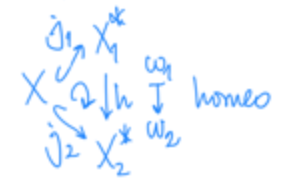
\includegraphics[scale=0.3]{images/comp_pto_prop_1} 
    \end{center}
\end{enumerate}
\end{prop}
\begin{demo}
\begin{enumerate}
    \item $X^* = X \cup \{0\},\ \mathcal{T}^* = \mathcal{T} \cup \{X^* \setminus K: \overbrace{K}^{\subset X} \text{comp.}\}$.
    \begin{itemize}
        \item $\mathcal{T}^*$ es top: fácil por las hipótesis sobre $X$.
        \begin{itemize}
            \item $K_i \stackrel{\text{comp.}}{\subset} X \xRightarrow{T_2} K_i \cerr X \Rightarrow \overbrace{\bigcap_{i} K_i}^{\text{cerr.}} \subset \overbrace{K_{i_0}}^{\text{comp.}} \Rightarrow \bigcap_{i} K_i$ comp.
            \item $U \ab X,\ X \stackrel{\text{comp.}}{\subset} X \Rightarrow U \setminus K =$ ab. $\setminus$ cerr. $ = $ ab.
            \item $U \ab X,\ K \stackrel{\text{comp.}}{\subset} X \Rightarrow U \cup \left( X^* \setminus K \right) = X^* \setminus \left( K \setminus U \right),\ K \setminus U \subset K$ cerrado $\Rightarrow$ compacto.
        \end{itemize}
        \item $X \subset X^*$ inmersión abierta: $\left( X^* \setminus K \right) \cap X = X \setminus K \in \mathcal{T}$ pues $X$ es $T_2$.
        \item $X^*$ es compacto: $X^* = \bigcup_{i} W_i$.
        \[
        \exists W_{i_0} \ni w \Rightarrow W_{i_0} = \underbrace{X^* \setminus K}_{\text{comp.}} \Rightarrow K \subset W_{i_1} \cup \ldots \cup W_{i_r} \Rightarrow X^* = W_{i_0} \cup W_{i_1} \cup \ldots \cup W_{i_r}  
        \]
        \item $X^*$ es $T_2:$
        \[
        x \in X \text{ loc. comp.} \Rightarrow \exists K^x \text{ ent. comp.} \Rightarrow X^* \setminus K^* = U^w \text{ ent. de } w
        \]
    \end{itemize}

    \item Unicidad:
    \begin{itemize}
        \item $\begin{rcases}
           h_{j_1} = j_2\\
           j_i \text{ inmersiones} 
        \end{rcases} \Rightarrow h|: j_1\left( X \right) \rightarrow j_2 \left( X \right)$ homeomorfismo.

        \item $h$ continua en $w_1$ (análogamente $h^{-1}$ continua en $w_2$)
        \begin{align*}
            h\left( w_1 \right) = w_2 \in W \ab X_2^* &\Rightarrow X_2^* \setminus W \cerr X_2^* \Rightarrow X_2^* \setminus W \stackrel{\text{comp.}}{\subset} j_2\left( X \right)\\
            &\Rightarrow K = h^{-1}\left( X_2^* \setminus W \right) \stackrel{\text{comp.}}{\subset} j_1\left( X \right) \subset X_1^*\\
            \left[ X_1^* \text{ es } T_2 \right] &\Rightarrow K \cerr X_1^* \Rightarrow h^{-1}\left( W \right) = X_1^* \setminus K \ab X_1^*
        .\end{align*}
    \end{itemize}
\end{enumerate}
\end{demo}

\begin{defi}
El espacio $X^*$ se denomina \underline{compactificación por un punto} de $X$. 

También, \underline{compactificación de Alexandroff}.
\end{defi}
Por ejemplo, $\mathbb{S}^n$ es la compactificación por un puntoo de $\mathbb{R}^n$ (vía proyección estéreo como dijimos antes).

\begin{obs}[¡Importante!]
\begin{enumerate}
    \item La unicidad justifica? que un espacio $X^*$ compacto $T_2$ es la compactificación de $X^* \setminus \{0\}$ para cualquier $w \in X^*$.

    \item Si dos espacios son homeomorfos, lo son sus compactos.
    \[
        X_1 \xrightarrow[\text{homeo.}]{f} X_2 \xhookrightarrow{j_2} X_2^* \Rightarrow j_1 = j_2 \circ f : X_1 \rightarrow X_2^*
    \]
    que cumple las condiciones.

    \item Si dos espacios no son homeomorfos, pueden serlo sus compactos.
    \begin{center}
        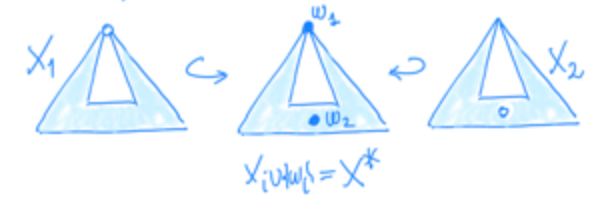
\includegraphics[scale=0.3]{images/obs_comp_pto} 
    \end{center}
\end{enumerate} 
\end{obs}

[\underline{Ejercicio}: $\mathbb{R}_u^2$: ¿Por qué $X_1 \not \approx X_2$?]
